\documentclass{beamer}
\usepackage{array}
\usepackage{xcolor}
\usecolortheme{magpie}
\title{Models for Antibody Data}
\date{}
\begin{document}

\begin{frame}
	\titlepage
\end{frame}

\section{Data}

\begin{frame}{test 1}
\frametitle{Data example}
	\begin{table}
	\begin{tabular}{cc}
		Infection status & Antibody titre \\
		\hline
		1 & 5 \\
		0 & 20 \\ 
		0 & 40 \\ 
		1 & 10 \\ 
		0 & 80 \\
		... & ... 
	\end{tabular}
	\end{table}

\end{frame}

\section{Model curves}

\begin{frame}
\frametitle{Probability profiles}
	
	\begin{figure}
		\includegraphics<1>[scale = 0.75]{../curve-models/curve_0_dark.pdf}%
		\includegraphics<2>[scale = 0.75]{../curve-models/curve_1_dark.pdf}%
		\includegraphics<3>[scale = 0.75]{../curve-models/curve_2_dark.pdf}%
		\includegraphics<4>[scale = 0.75]{../curve-models/curve_2_dark.pdf}%
		\includegraphics<5>[scale = 0.75]{../curve-models/curve_3_dark.pdf}%
		\includegraphics<6>[scale = 0.75]{../curve-models/curve_4_dark.pdf}%
		\includegraphics<7>[scale = 0.75]{../curve-models/curve_4_dark.pdf}%
		\includegraphics<8>[scale = 0.75]{../curve-models/curve_5_dark.pdf}%
		\includegraphics<9>[scale = 0.75]{../curve-models/curve_6_dark.pdf}%
		\includegraphics<10>[scale = 0.75]{../curve-models/curve_6_dark.pdf}%
	\end{figure}
	
	\pause
	\pause
	\pause
	
	\begin{table}
	\begin{tabular}{l | ccc}
		 & Top & Bottom & Change \\
		\hline
		Logistic & Fixed at 1 & Fixed at 0 & S-shape \pause \pause \pause \\
		Scaled logistic & Estimated & Fixed at 0 & S-shape \pause \pause \pause \\
		Cox PH & Not estimated & Not estimated & Exponential
	\end{tabular}
	\end{table}

\end{frame}

\section{Cox model}

\subsection{Cox model data}

\begin{frame}
\frametitle{Cox model data}
	\begin{table}
	\begin{tabular}{cc<{\onslide<2->}c<{\onslide}}
		Infection status & Antibody titre & Time \\
		\hline
		1 & 5 & 78 \\
		0 & 20 & 97 \\ 
		0 & 40 & 85 \\ 
		1 & 10 & 110 \\ 
		0 & 80 & 133 \\
		... & ... & ...
	\end{tabular}
	\end{table}
\end{frame}

\subsection{Cox model time}

\begin{frame}
\frametitle{Cox model time}

	
	\begin{figure}
		\includegraphics<1>[scale = 0.75]{../curve-cox/timeplot_0_dark.pdf}%
		\includegraphics<2-3>[scale = 0.75]{../curve-cox/timeplot_1_dark.pdf}%
		\includegraphics<4>[scale = 0.75]{../curve-cox/timeplot_2_dark.pdf}%
	\end{figure}
	
	\pause
	\pause
	
	Cox model assumes that time is: time \textcolor{yellow}{at risk} of an \textcolor{yellow}{observable} event.
	
\end{frame}

\begin{frame}
\frametitle{Cox model time}
	
	\begin{figure}
		\includegraphics[scale = 0.75]{../curve-cox/timeplot_2_dark.pdf}%
	\end{figure}
	
	Not necesarily a problem with an additional assumption. \pause
	
	Time of follow-up is proportional to time at risk.
	
\end{frame}

\section{Logistic regression}

\begin{frame}
\frametitle{Logistic regression}

	\begin{figure}
		\includegraphics[scale = 0.75]{../curve-models/curve_2_dark.pdf}%
	\end{figure}

	\begin{table}
	\begin{tabular}{l | ccc}
		 & Top & Bottom & Change \\
		\hline
		Logistic & Fixed at 1 & Fixed at 0 & S-shape
	\end{tabular}
	\end{table}

\end{frame}

\begin{frame}
\frametitle{Logistic regression}

	\begin{figure}
		\includegraphics[scale = 0.75]{../curve-models/curve_2_dark.pdf}%
	\end{figure}

	\begin{table}
	\begin{tabular}{l | ccc}
		 & Top & Bottom & Change \\
		\hline
		Logistic & \textcolor{yellow}{Fixed at 1} & Fixed at 0 & S-shape
	\end{tabular}
	\end{table}

\end{frame}

\begin{frame}
\frametitle{Hanam cohort --- everyone}

	\begin{figure}
		\includegraphics[scale = 0.7]{../data-plot/hanam_scatter_general_dark.pdf}%
	\end{figure}

\end{frame}

\begin{frame}
\frametitle{Hanam cohort --- exposed}

	\begin{figure}[t]
		\includegraphics[scale = 0.7]{../data-plot/hanam_scatter_dark.pdf}%
	\end{figure}

\end{frame}

\begin{frame}
\frametitle{Logistic fit}
	
	\begin{figure}
		\includegraphics<1>[scale = 1]{../logistic-plot/lrex_pres1.pdf}%
		\includegraphics<2>[scale = 1]{../logistic-plot/lrex_pres2.pdf}%
		\includegraphics<3, 7>[scale = 1]{../logistic-plot/lrex_pres3.pdf}%
		\includegraphics<4>[scale = 1]{../logistic-plot/lrex_pres4.pdf}%
		\includegraphics<5>[scale = 1]{../logistic-plot/lrex_pres5.pdf}%
		\includegraphics<6>[scale = 1]{../logistic-plot/lrex_pres6.pdf}%
		\includegraphics<8>[scale = 1]{../logistic-plot/lrex_pres7.pdf}%
		\includegraphics<9>[scale = 1]{../logistic-plot/lrex_pres8.pdf}%
	\end{figure}

\end{frame}

\section{Relative protection}

\begin{frame}
\frametitle{Relative protection curve}

\pause
	
	\begin{itemize}
		\item Unreliable with logistic regression
		\pause
		\begin{itemize}
			\item Derived from fitted infection probabilities
			\pause
			\item Titre of 5 is not a real measurement
		\end{itemize}
		\pause
		\item Unnecessary with scaled logistic regression
		\pause
		\begin{itemize}
			\item Estimates baseline
		\end{itemize}
	\end{itemize}

\end{frame}

\section{Scaled logit}

\begin{frame}
\frametitle{Scaled logistic regression}

	\begin{figure}
		\includegraphics[scale = 0.75]{../curve-models/curve_7_dark.pdf}%
	\end{figure}

	\pause

	\begin{table}
	\begin{tabular}{l | ccc}
		 & Top & Bottom & Change \\
		\hline
		Scaled logistic & Estimated & \textcolor{yellow}{Fixed at 0} & \textcolor{yellow}{S-shape}
	\end{tabular}
	\end{table}

\end{frame}

\begin{frame}
\frametitle{Scaled logistic regression}

	\begin{figure}
		\includegraphics[scale = 0.6]{../data-plot/hanam_counts_general_dark.pdf}%
	\end{figure}

	\begin{table}
	\begin{tabular}{l | ccc}
		 & Top & Bottom & Change \\
		\hline
		Scaled logistic & Estimated & \textcolor{yellow}{Fixed at 0} & \textcolor{yellow}{S-shape}
	\end{tabular}
	\end{table}

\end{frame}

\begin{frame}
\frametitle{Scaled logistic regression}
\onslide<2>{Maximum likelihood to midpoints}

	\begin{figure}
		\includegraphics<1>[scale = 0.6]{../data-plot/hanam_counts_general_dark.pdf}%
		\includegraphics<2>[scale = 0.6]{../fit-sclr/infection-boot_dark.pdf}%
	\end{figure}

	\begin{table}
	\begin{tabular}{l | ccc}
		 & Top & Bottom & Change \\
		\hline
		Scaled logistic & Estimated & Fixed at 0 & \textcolor{yellow}{S-shape}
	\end{tabular}
	\end{table}

\end{frame}

\begin{frame}
\frametitle{Scaled logistic regression}
\onslide<1>{Bayesian}

	\begin{figure}
		\includegraphics<1>[scale = 0.6]{../fit-bayesian-plot/infection_dark.pdf}%
	\end{figure}

	\begin{table}
	\begin{tabular}{l | ccc}
		 & Top & Bottom & Change \\
		\hline
		Scaled logistic & Estimated & Fixed at 0 & \textcolor{yellow}{S-shape}
	\end{tabular}
	\end{table}

\end{frame}

\begin{frame}
\frametitle{Models}
	\pause
	\begin{table}
	\begin{tabular}{l | ccc}
		Cox PH & \pause Requires an additional assumption \pause \\
		Logistic & Assumption not satisfied \pause \\
		Scaled logistic & Requires a larger sample size
	\end{tabular}
	\end{table}
\end{frame}

\end{document}